\chapter{History}
\label{ch:history}
\section{The Phenomenon of Spin}

Spin is a fundamental quantity possessed by all elementary particles. The word
`spin' is used to describe the property because particles which possess spin
behave as though they have some kind of intrinsic hidden rotation, as if they
were `spinning'. The dimension of spin is angular momentum. Spin is somewhat
bizarre, because one does not observe anything physically spinning, although
there are some phenomena (such as orbital angular momenta) which can be naively
thought of as a `spinning system'. For quantum mechanical systems, the classical
analogy breaks down since a system's spin is a superposition of possible spin
states.  The role of spin in physics is of foundational importance, therefore
physicists should strive  to understand origin of spin in the building blocks of
the visible universe--protons and neutrons.

Relativistic particles that possess non-zero spin are chiral (handed).  The
existence of Chirality has huge implications for how elementary particles can
generate structure in matter itself~\cite{Brodsky1988}. In the case of the weak
interaction, the presence of spin creates chiral spinors that break the
left-right symmetry of weak coupling in matter. This symmetry breaking is
exploited in this thesis to probe the spin of the proton sea.

The phenomena of spin also imposes rules for how ensembles of particles may
exist in a potential. Particles with spin are fermions. Because these particles
must obey Fermi-statistics, structure is observed in all the visible matter of
the universe. Without spin, the world as we know it would collapse in on itself,
making any kind of extended non-exotic structures which currently exist by
virtue of the Pauli exclusion principal, impossible.

\clearpage
\section{A Brief History of Relevant Physics}

The study of spin is an outgrowth of the general study of matter.  Models
for matter, and the underlying structure of matter (in the modern sense),
represent over a hundred years of experimental and theoretical efforts, and
thousands of years of contemplating what makes up the universe.

Although indulgent on my part, I find it interesting and humbling to try and map
out the path that humanity and science has trodden on its way to understanding
the building blocks of the universe. To find the first time that humanity began
to realize that our visible world is constructed from invisible, fundamental
building blocks, we must travel back nearly 2,500 years into the past.

\section{Ancient Foundations} 

Sometime between 490 - 370 BCE lived two philosophers, Empedocles (Figure
~\ref{fig:empedocles}), and Democritus (Figure~\ref{fig:democritus}). Both men
lived approximately at the same time and made huge philosophical leaps in
attempting to understand the nature of the visible world.

\begin{figure}[ht]
	\centering
	\begin{subfigure}{.5\textwidth}
		\centering
		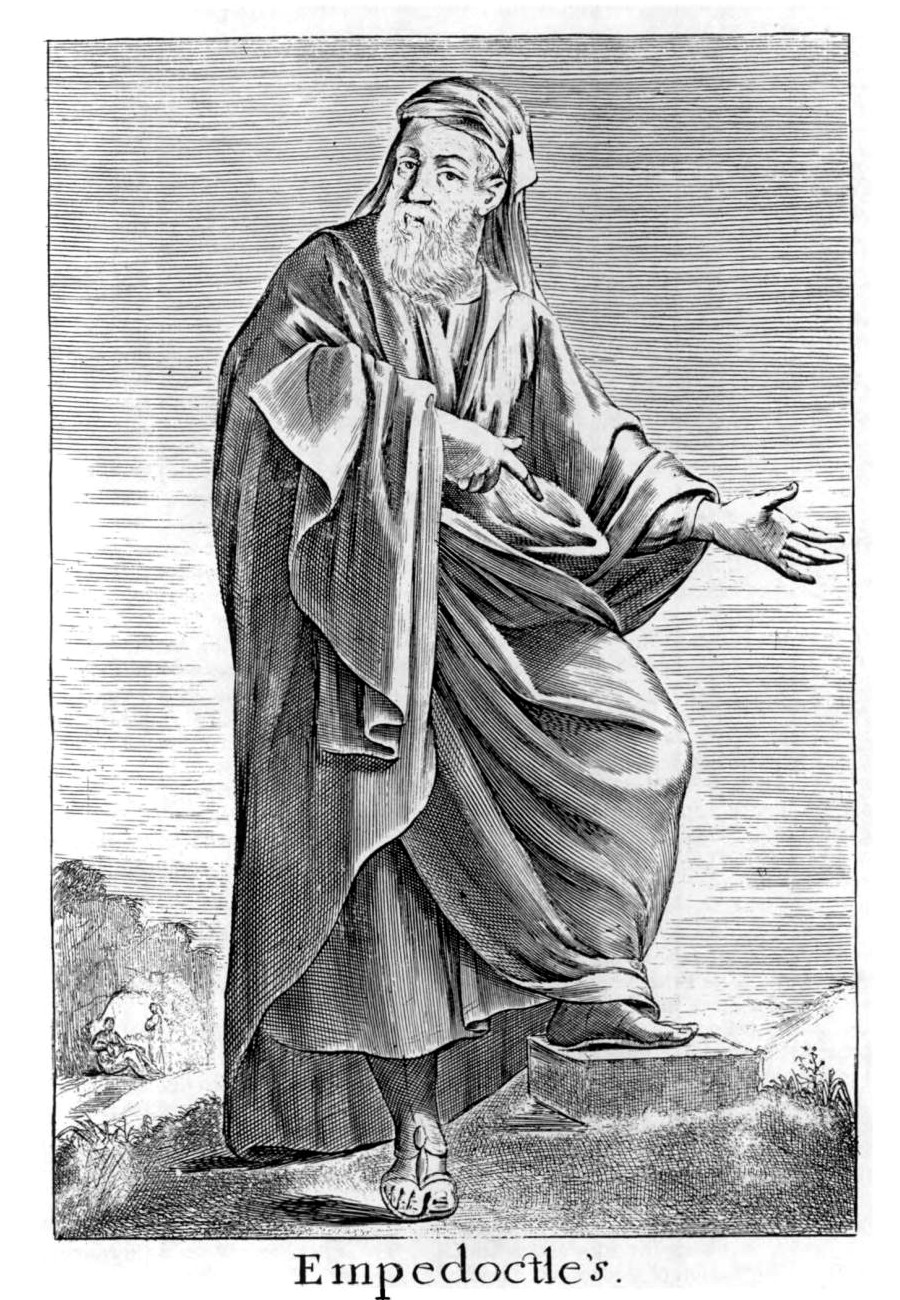
\includegraphics[width=0.4\linewidth]{./figures/empedocles.jpg}
		\caption{Empedocles \cite{Stanley1655}}
		\label{fig:empedocles}
	\end{subfigure}%
	\begin{subfigure}{0.5\textwidth}
		\centering
		
\includegraphics[width=0.4\linewidth]{./figures/democritus.jpg}
		\caption{Democritus \cite{Brugghen1628}}
		\label{fig:democritus}
	\end{subfigure}
  \caption{ 
    Two Greek philosophers, who made important philosophical contributions our
    understanding of matter. Empedocles (Panel (a)), postulated the precursor
    to the elemental theory of matter\cite{Long1949} and Democritus (Panel
    (b)), postulated the precursor to the atomic theory of matter.  
  }
	\label{fig:atomists}
\end{figure}

Democritus was part of a movement of thought which was first to make the
intellectual jump that perhaps matter was not a continuum, but instead composed
of `atomon'. `Atomon' were thought to be small and indivisible particles
building up all that is observable~\cite{Baldes1978}.  Empedocles made an
equally important philosophical stride--he posited that matter must be composed
of elemental primitives and that the properties of the primitives which build
up matter, influence the properties of the bulk matter itself~\cite{Long1949}.

Although Empedocles' `periodic table' was only composed of Earth, Water, Fire,
and Air, the idea that some unseen transmutation of elemental forces might
generate observables in nature was an important step forward. This was the
first time that humans considered that underlying structure in matter might
influence the bulk properties of matter. Proto-scientists were beginning to
generate models which derived our complicated observations from simpler forms.

\clearpage
\section{The Scientific Revolution}

Thanks to the mathematical foundations laid out by the minds of the Islamic
Golden Age (8th century - 13th century), Europe was well poised to reignite the
flames of scientific inquiry during the post Renaissance Scientific
Revolution~\cite{Alexakos2005} (17th - 18th centuries), following a renewed
interest the ideas of Greek philosophers after the dark ages.

The Scientific Revolution represented an unprecedented period of growth in
science, thanks the foundations laid during the Italian Renaissance and
emergence of British Empiricism~\cite{Cowley1968}.

\begin{figure}[ht]
	\centering
	\begin{subfigure}{.5\textwidth}
		\centering
		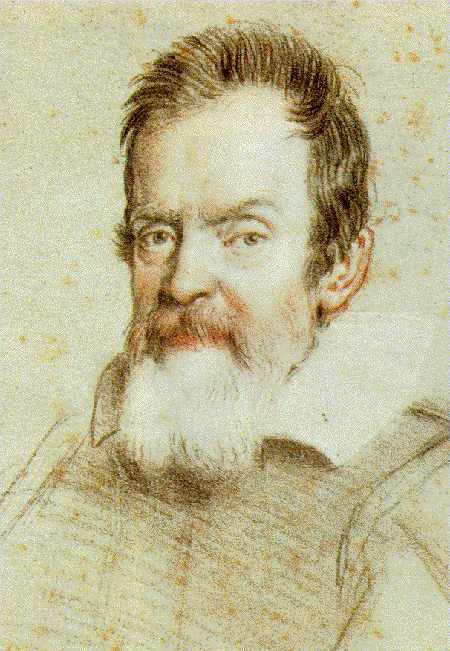
\includegraphics[width=0.4\linewidth]{./figures/galileo.jpg}
		\caption{Galileo \cite{Leoni1624}}
		\label{fig:galileo}
	\end{subfigure}%
	\begin{subfigure}{0.5\textwidth}
		\centering
		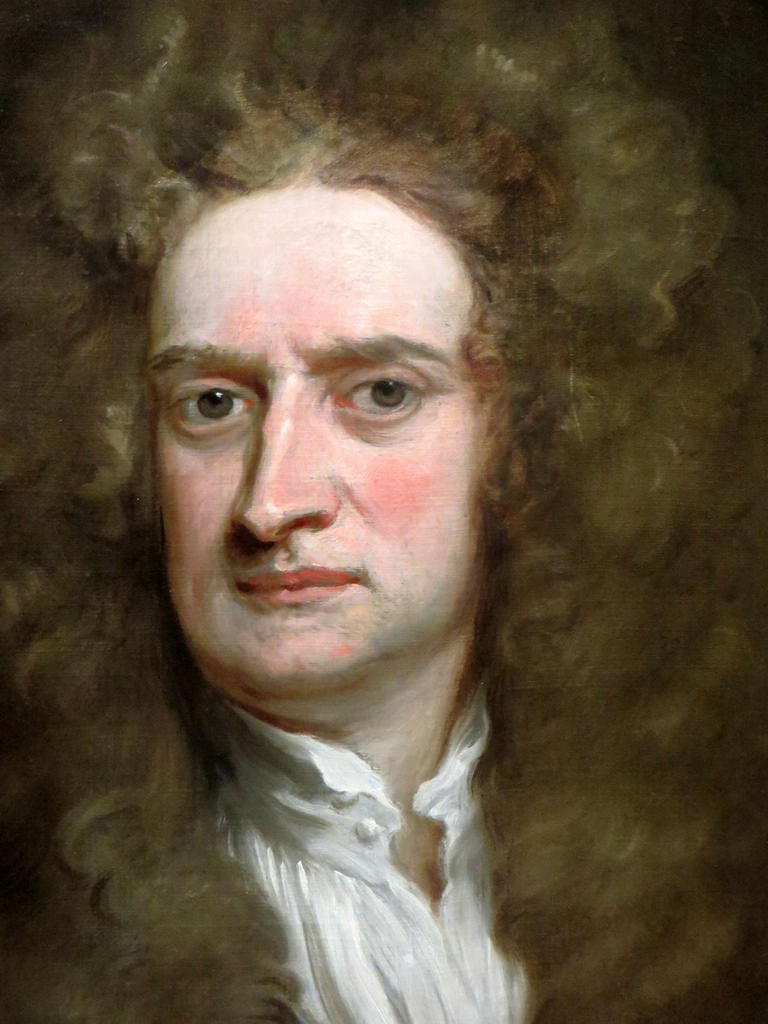
\includegraphics[width=0.4\linewidth]{./figures/newton.jpg}
		\caption{Newton}
		\label{fig:newton}
	\end{subfigure}
	\caption{ 
    Giants in the age of Empiricism, Newton (Panel (a)) and Galileo (Panel (b))
    both made foundational contributions to Physics.  Galileo lived in Italy,
    born in 1564 and dying in 1642. Newton lived in England from 1642 until his
    death in 1727
	}
	\label{fig:newtongalileo}
\end{figure}

\subsection{Galileo Galilei}

Coming at the tail end of the Italian Renaissance, Galileo brought us into the
age of Scientific Revolution.

While Galileo is best known for his work in Observational Astronomy, his
importance to science extends beyond this. During his years in exile for his
controversial views regarding the heliocentric universe, he produced some of
his most important scientific work in kinematics~\cite{Hall1965}. What made
this work remarkable is the care that Galileo took in merging mathematical
modeling with well designed experimentation. This methodical approach to
inquiry laid the foundation for the scientific method, which others would
refine. 

Galileo's formalization of the scientific method inexorably set science on a
course to delving deep into the nature of matter and the laws of nature.

\subsection{Isaac Newton}

Fittingly born in the same year as Galileo's death, Isaac Newton would carry on
Galileo's legacy of rigorous mathematical modeling mixed with experimentation.
Perhaps no other scientist has touched so many different aspects of physics,
from theories of propagation of light, to celestial mechanics, to mathematics,
and kinematics.

Newton's Principia is arguably the most important scientific work ever
published.  It opened the doors of the universe in a way that nobody has since
duplicated--Newtons' laws of motion are still taught in school today, and
applied in real scientific contexts, providing the basis for the NASA space
exploration program. Although Newton's models for motion have since been shown
to be inaccurate at the smallest and largest scales, they still provide
startlingly accurate predictions at intermediate scales.

One particularly prescient theory of Newton's was his corpuscular theory of
light. Although not his most influential theory by far, the idea that an
apparently continuous medium such as a beam of light might be made of small
packets of energy (corpuscles) turned out to be partially
right~\cite{Stuewer1970}, and gained an interesting new context with the
emergence of Quantum Mechanics in the early 20th century.

Newton's theories, and contributions to science are enormous, and have moved us
deeper still into the underpinnings of matter. It would not be until roughly 200
years after his death, in the 19th century, that we finally can take the first
steps into the world of the atomic, and sub-atomic: the world of the proton. 

\clearpage
\section{Atomic Theory}

On the shoulders of giants such as Newton and Galileo, science finally came to
know the tool which has been indispensable to modern particle physics:
scattering. Rutherford and Thompson both carried out the most important
scattering experiments in modern science. These experiments provided us with
the first hints of a hidden, quantum world. It would not be until the 20th
century that these important experiments would be fully contextualized with a
theory of quantum scattering.

Scattering experiments offer a very powerful method where one uses a well known
initial state of matter (typically in the form of a beam) and allows this beam
to interact with an unknown configuration of matter. The final state of the
target and scattered beam are measured. With a careful study of the kinematics
of the scattered beam, one can create models that offer a peak into the
structure of the target matter. As we journey down further in scale, matter
begins to look quite different.  In fact, the models we use are scale dependent
as seen in Figure~\ref{fig:scale_of_matter}. Thomson
(Figure~\ref{fig:thomsonrays}), and Rutherford (Figure~\ref{fig:rutherford})
began to see matter as collections of atoms.  Soon, nuclei were discovered to be
divisible into protons an neutrons, which in turn were discovered to be composed
of a sea of quarks and gluons.

\begin{figure}[ht]
	\centering
	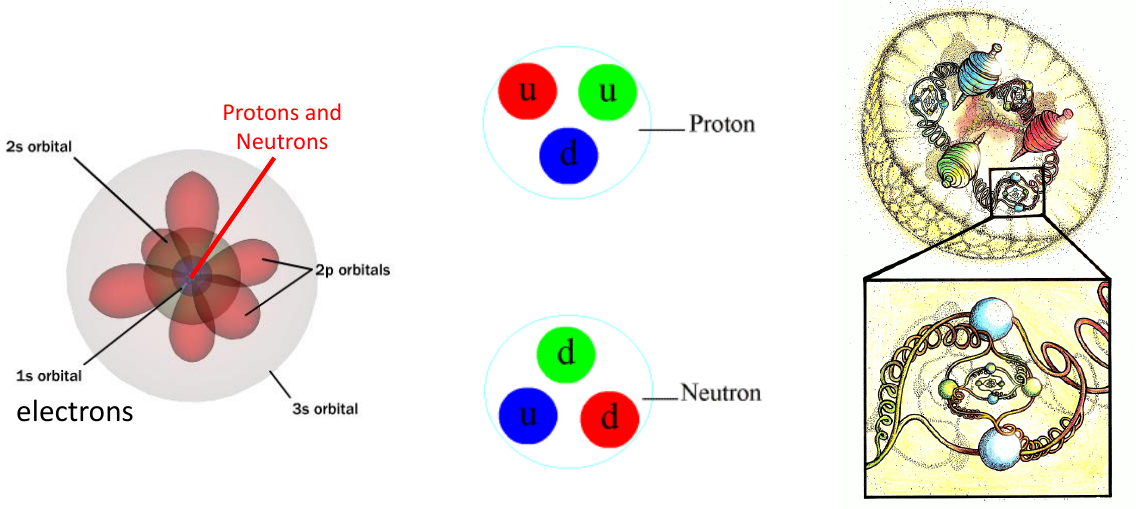
\includegraphics[width=\linewidth]{./figures/scale_of_matter.png}
	\caption{
    Matter at an atomic scale~\cite{Freudenrich2001} (left), intermediate
    nuclear scale~\cite{Manisearth2010} (center), and the sub-nuclear partonic
    scale (right)~\cite{Morreale2009}
	}
	\label{fig:scale_of_matter}
\end{figure}

\subsection{John Dalton}

While many had postulated the existence of atoms, the first evidence based
theory which suggested the existence of atoms was produced by John Dalton in the
early 19th century. Dalton made an important conceptual leap to relate the
existence of stoichiometric ratios in chemistry to the presence of small,
individual functional units in his experiments with chemical reactions.
Dalton's realization was only made possible due to his careful accounting of
reactants in his experiments.

However, humanity had to wait for Einstein's 1905 theory on Brownian Motion to
be experimentally verified by Jean Perrin to obtain the first limits on the mass
and size of atoms that Dalton's atomic theory predicted~\cite{Patterson200750}.

\subsection{J.J. Thompson}

\begin{figure}[ht]
	\centering
	\begin{subfigure}{.4\textwidth}
		\centering
		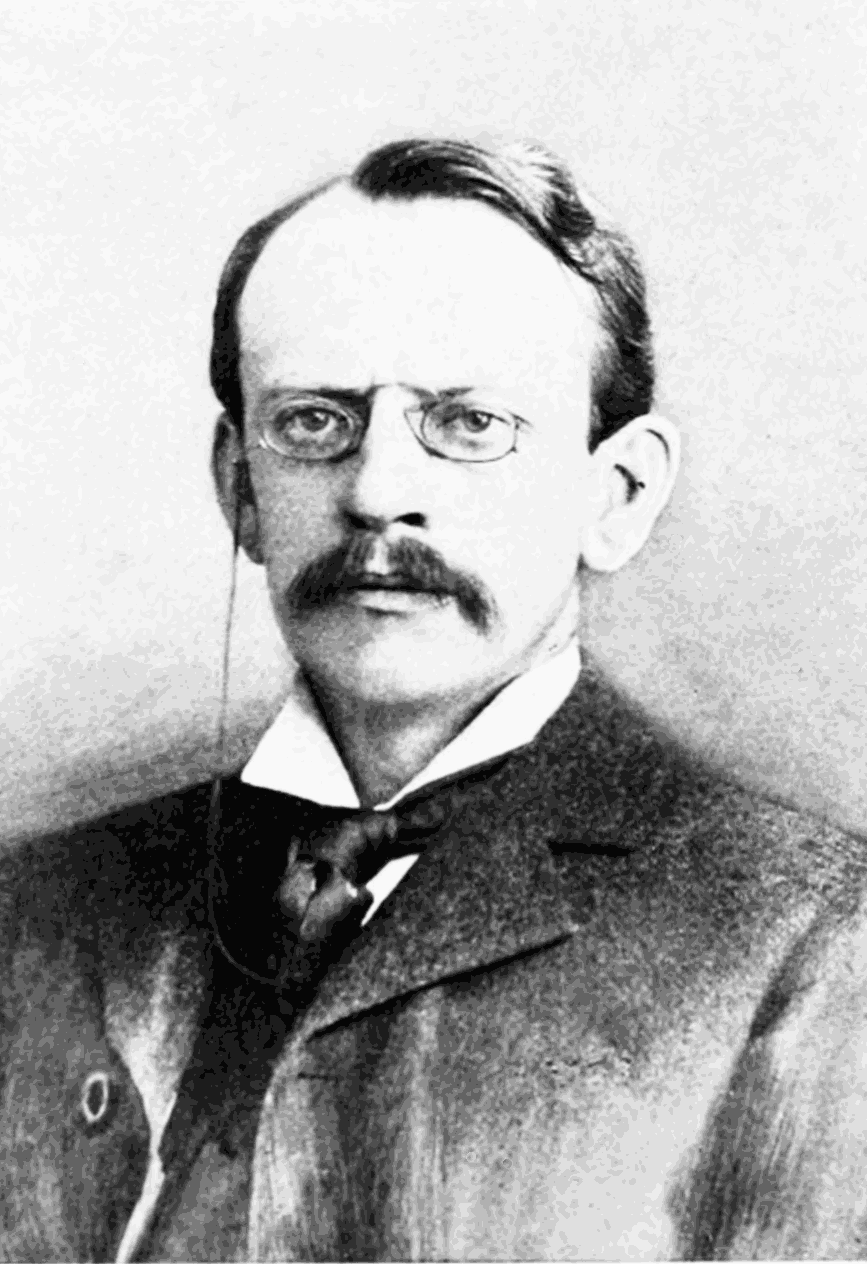
\includegraphics[width=0.4\linewidth]{./figures/jjthomson.png}
		\caption{J.J. Thomson  \cite{PopularScience1899}}
		\label{fig:thomsonportrait}
	\end{subfigure}%
	\begin{subfigure}{0.6\textwidth}
		\centering
		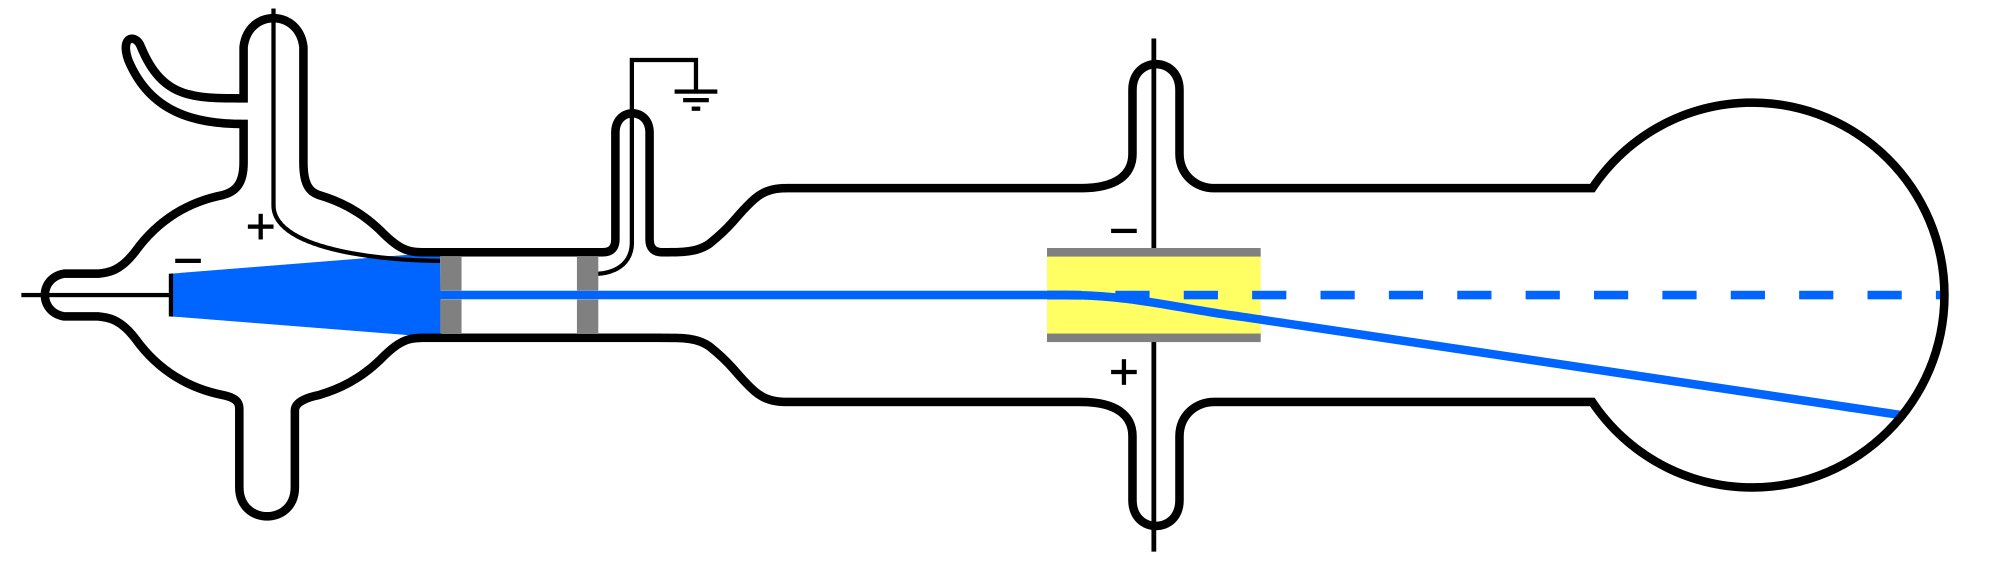
\includegraphics[width=0.4\linewidth]{./figures/cathoderaytube.png}
		\caption{Cathode Ray Tube  \cite{Kurzon2010}}
		\label{fig:thomsoncathode}
	\end{subfigure}
	\caption{ 
		Left: J.J. Thomson, who showed that cathode ray tubes were in fact producing
		the first observed subatomic particle: the electron. Right: A cartoon of
		Thomson's cathode ray tube setup. Electrons would be deflected by a magnetic
		field, sent from cathode to anode.
	}
	\label{fig:jjthomson}
\end{figure}

Thomson (Figure~\ref{fig:jjthomson}) would discover that atoms are not the
smallest indivisible piece of matter. In his landmark experiment, he used
cathode ray scattering experiments to show that cathode rays were in fact
subatomic particles. He showed these cathode rays were identical to particles
given off by the photoelectric effect. He discovered that these were the same
particles responsible for electric current.  Scientists began to wonder: if
atoms were not the smallest piece of matter, then perhaps atoms themselves
might not be `indivisible' as previously thought \cite{nobelthomson2014}.

\subsection{Ernest Rutherford}

\begin{figure}[ht]
	\centering
	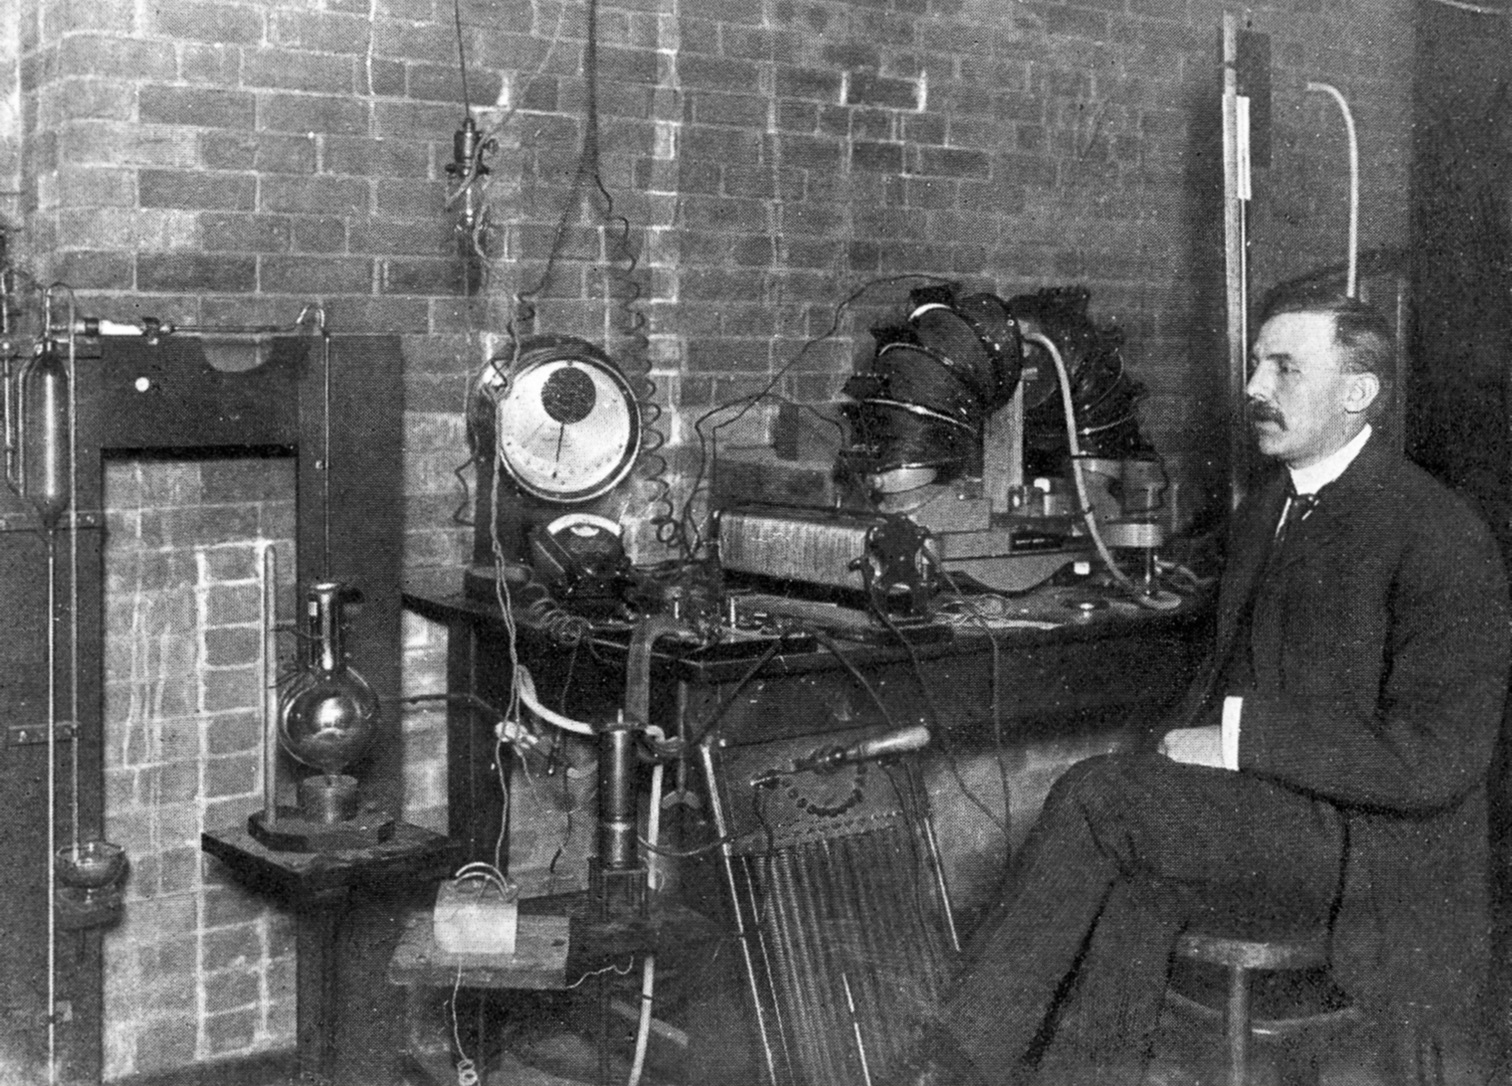
\includegraphics[width=0.6\linewidth]{./figures/ernestrutherford.jpg}
	\caption{Ernest Rutherford, in his lab.  \cite{Eve1939}}
	\label{fig:rutherford}
\end{figure}

Ernest Rutherford (Fig~\ref{fig:rutherford}) was the first to show that atoms
themselves had underlying structure and consisted of a small dense center.  He
had discovered the nucleus.

\begin{figure}[ht]
	\centering
	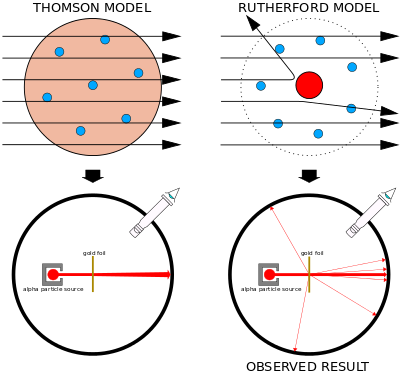
\includegraphics[width=0.6\linewidth]{./figures/geiger_marsden.png}
	\caption{
		Ernest Rutherford's historic experiment, showing (top right) that atoms were
		composed of a small dense nucleus, in contrast to Thomson's `pudding model'
		of homogeneous charge (top left). The experiment, (bottom left and right)
		contrast the expected results (bottom left) against the observed results
		(bottom right)  \cite{Kurzon2014}.
	}
	\label{fig:geigermarsden}
\end{figure}

Rutherford's work with radioactivity was of fundamental importance. He
discovered and classified both alpha-particle radioactivity and beta-particle
radioactivity. Further studies into these types of nuclear radiation would
unlock the nucleus of atoms through the work of future scientists.

After his discovery of the proton, Rutherford proposed a planetary model for the
nucleus. While this model was eventually shown to be wrong, it shifted paradigms
from the pudding model of atoms to the more familiar nucleus + electron model.
This shift eventually led to the emergence of Quantum Mechanics.

Rutherford's work helped push us out of the cocoon of classical mechanics into
the world of the quantum mechanics--scientists would soon find that the nucleus
is not just a dense concentration of charge, but a probabilistic structure, with
rich sub nuclear structure.

\clearpage
\section{Early Quantum Theory}

During Rutherford's time, experiments were already underway investigating
modeling light as a wave phenomena. This was in contrast to Newton's
(unverified) corpuscular theory of light. The argument whether light was
wave-like or particle-like eventually lead to a classical field theory
describing light as electromagnetic radiation. Max Planck proposed theories
which required the quantization of light~\cite{Planck1901}.  Einstein would show
that light is indeed quantized into packets of energy in his analysis of the
photoelectric effect. The nascent atomic theory of matter hinted at a hidden,
quantized world.

\begin{figure}
	\centering
	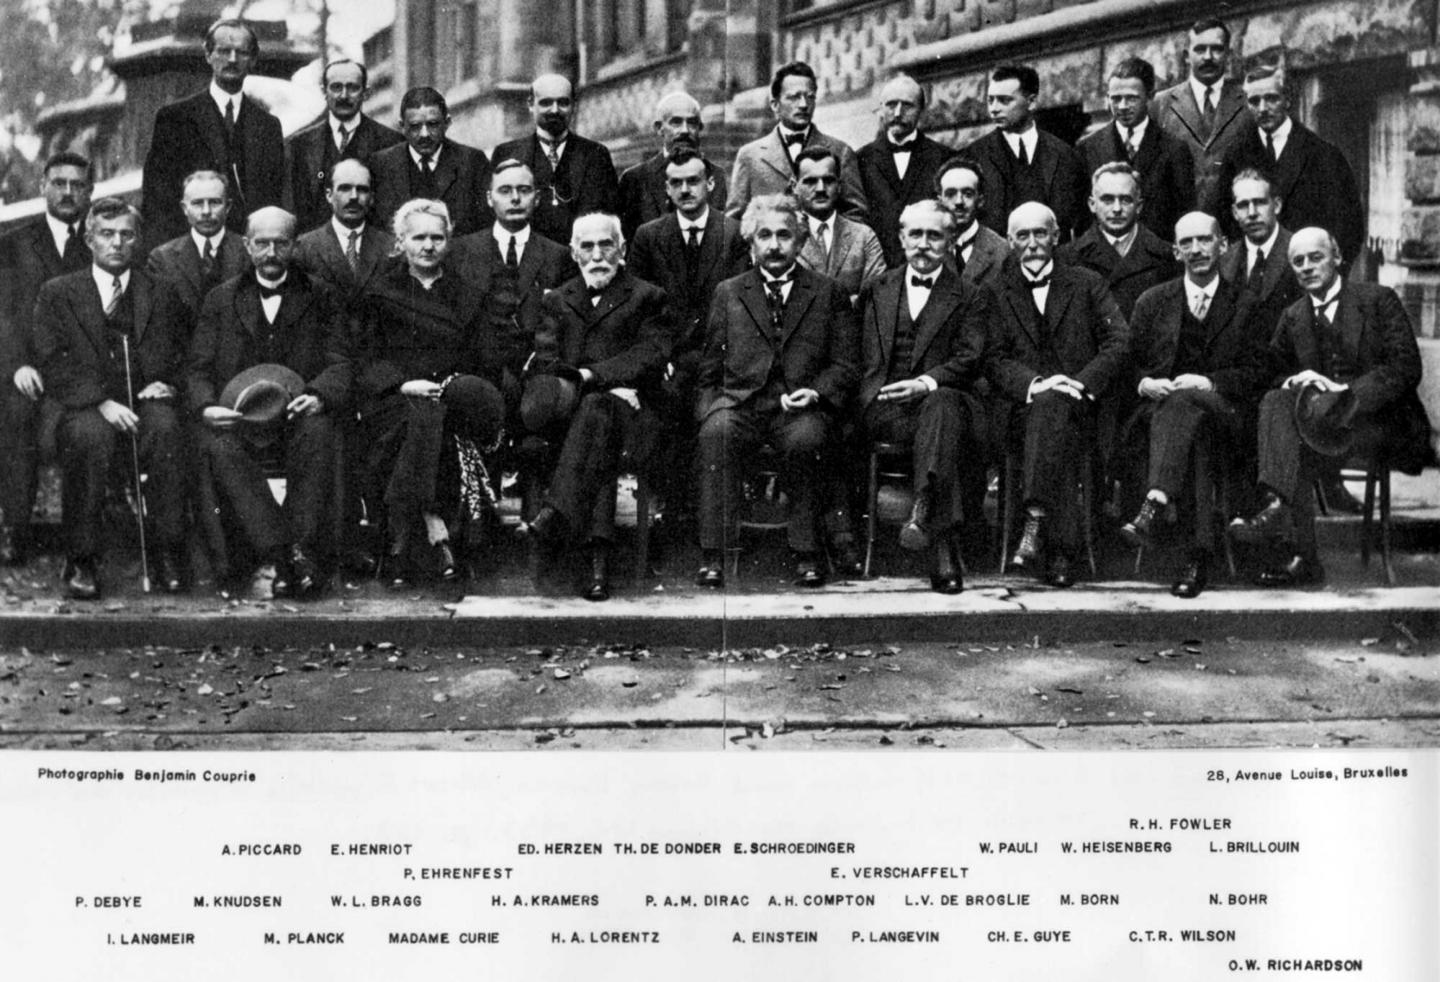
\includegraphics[width=\linewidth]{./figures/solvay.jpg}
	\caption{
		The attendees of the Solvay Conference in Brussels, 1927
		 \cite{BenjaminCroupie1927}.
	}
	\label{fig:solvay}
\end{figure}

At the 1927 Solvay Conference in Brussels (Figure~\ref{fig:solvay}) an
unprecedented gathering of some of the most important figures in modern physics,
built the foundations of what would become quantum mechanics. These scientists
defined the nature and rules of quantum mechanics--the weird model which
accommodates a wave-particle duality of matter. 

It was found that not only light possesses this wave-particle duality, but also
the particles that make up atoms. These models were formalized by Paul Dirac,
David Hilbert and John Von-Neumann.

Further refinements and additions to quantum mechanics gave birth to quantum
field theory. Early quantum models were very successful at describing static
particles trapped in static potentials. Scientists could predict exactly
observed atomic emission spectra. But, more work was needed to understand the
relationship between electrical currents, light and magnetism.  These concepts
were all related by James Clerk Maxwell~\cite{Maxwell1865} in the latter half of
the 19th century, but had yet to receive a quantum-treatment.

Dirac was first to create a model for describing the electron, its behavior in
electromagnetic fields, and photon emission and absorption. Dirac's models were
fully relativistic~\cite{Dirac}. Dirac's model was so successful, that it would
become the basis for what we now call quantum electrodynamics.  Much of the
mathematical formalism was reused to describe other field theories. Field Theory
is the ultimate language used in modeling and describing the structure of
matter--including the insides of a proton. 

\begin{figure}[ht]
	\centering
	\begin{subfigure}{.4\textwidth}
		\centering
		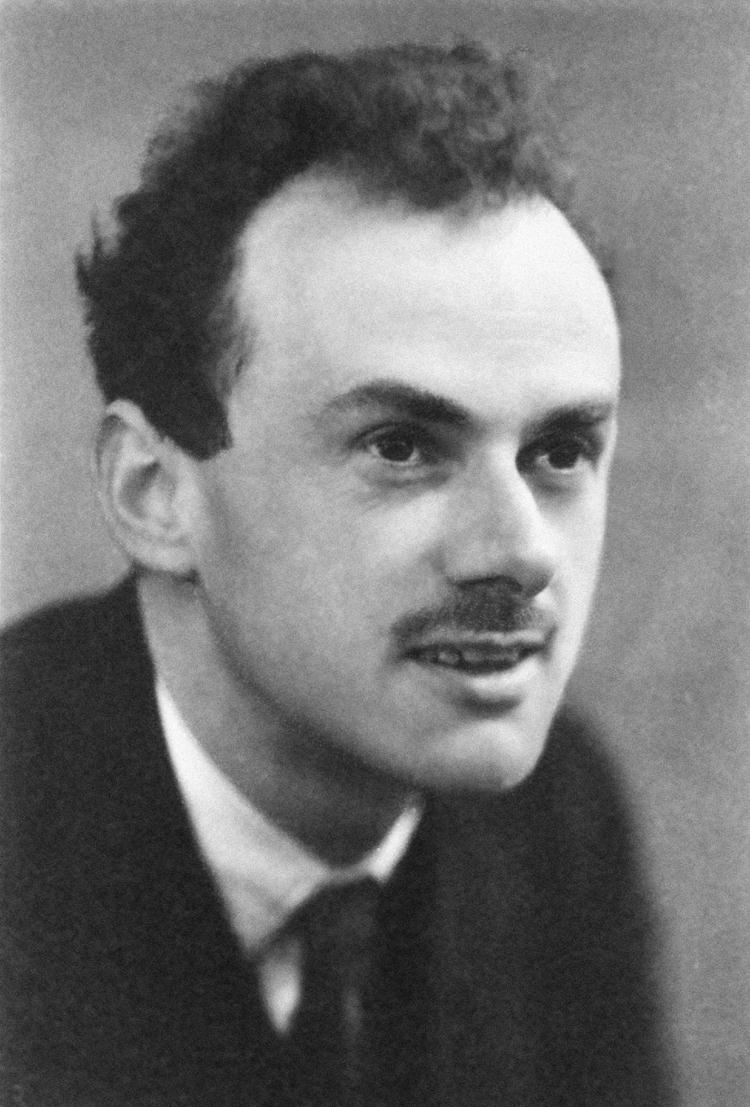
\includegraphics[width=0.4\linewidth]{./figures/pauldirac.jpg}
		\caption{Paul Dirac, 1933  \cite{NobelFoundation1933}}
		\label{fig:pauldirac}
	\end{subfigure}%
	\begin{subfigure}{0.6\textwidth}
		\centering
		\begin{equation}
			\left(\beta mc^2 + c\left(\sum_{n \mathop =1}^{3}\alpha_n p_n\right)\right) \psi (x,t) = i \hbar \frac{\partial\psi(x,t) }{\partial t}
		\end{equation}
		\caption{The `Original Form' of the Dirac Equation}
		\label{eq:diracquation}
	\end{subfigure}
	\caption{ 
		Paul Dirac, next to his original formulation of the Dirac Equation,
		describing the wave function for an electron with rest-mass $m$, in terms of
		its space-time coordinates. Dirac's equation has been expressed free of any
    defined basis.
	}
	\label{fig:thomsonrays}
\end{figure}

Dirac's work successfully merged relativity into his wave equations describing
the motion of particles. He additionally incorporated the spin (i.e. Dirac
Spinors) of these particles. The inclusion of spin allowed for the most precise
predictions ever to be made for hyperfine divisions in the atomic
spectra~\cite{Dirac}.

In Dirac's time, the proton was already known to reside in the enigmatic
nucleus. However attempts to use Quantum Electrodynamics to describe the state
of the nucleus failed. It was clear that there was a very strong force holding
together the positively charged protons of a nucleus. This force would have to
be far stronger than the electromagnetic repulsion felt by the positively
charged particles in such close proximity. Further complicating an understanding
of the nucleus is the fact that as the length scale of probing decreases, the
energies probed increase. This fundamentally makes the nucleus a relativistic
object. Physics would once again forge ahead in attempting to understand the
inner workings of the nucleus.

\clearpage
\section{Early Particle Physics and The Eightfold Way}

The hydrogen atom and its spectra was well-modeled with quantum mechanics by the
end of the early 20th century. However, attempts to study Helium were not as
successful. By 1932, when James Chadwick turned a beam of helium particles (at
that time only known as $\alpha$ particles) on a sample of Beryllium, he
observed that neutral, non-ionizing, penetrating radiation was produced
\cite{Krauss2015}.  Photons were ruled out as possible candidates, leading to
the discovery of the neutron. Protons and neutrons were hypothesized by
Heisenberg to both be the same state of a new conceptual particle, the
nucleon~\cite{Heisenberg1952}. In the same year, Carl Anderson discovered the
positron. 

By 1934, Hideki Yukawa (Fig.~\ref{fig:hidekiyukawa}) had created an effective
field theory for interactions of `elementary particles' (at this time, thought
to be protons and neutrons). He predicted the existence of mesons, and wrote
down an effective field theory which described how protons and neutrons bind
together in the nucleus \cite{Yukawa1935}. 

Though non-relativistic quantum mechanics was mostly complete by 1934,
scientists were already hard at work incorporating relativistic corrections to
the theory. Experiments with cosmic rays soon revealed the existence of muons
and the first observation of mesons.

\begin{figure}[ht]
	\begin{center}
		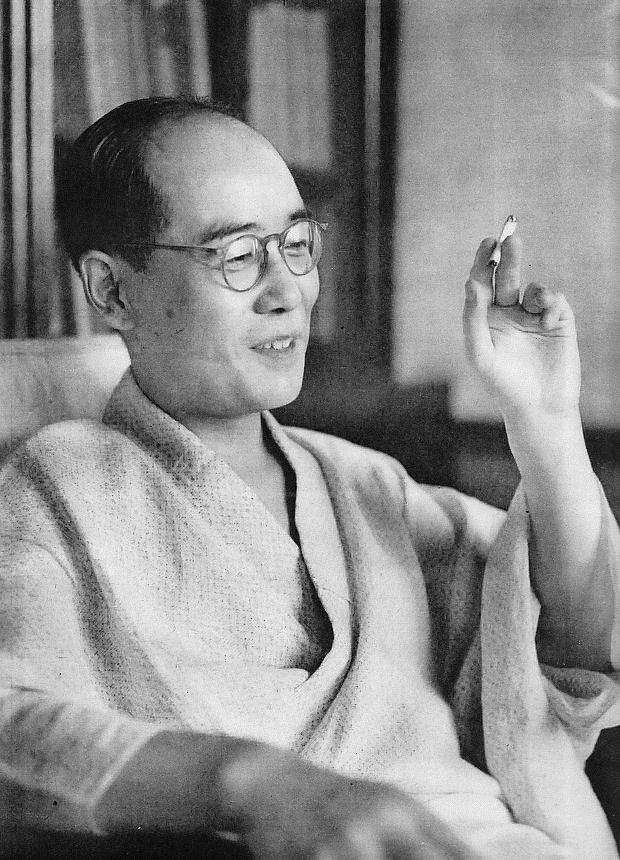
\includegraphics[width=0.5\linewidth]{./figures/hidekiyukawa.jpg}
		\caption{
			Hideki Yukawa, the first Japanese Nobel Laureate and publisher of
			influential research on the theory of mesons, and other elementary
			particles  \cite{YukawaPhoto1952}.
		}
		\label{fig:hidekiyukawa}
	\end{center}
\end{figure}

Three separate paths eventually lead to the development of particle
accelerators. To date, these massive machines provide the best apparatus in
physics to probe nuclear structure. These accelerators are an outgrowth of ever
more intense Rutherford-style experiments. An array of technologies have
supported this growth: Tandem Van-Der-Graaf generators, resonant acceleration
techniques, RF linacs, and betatron accelerators \cite{Bryant1994}.

By the 1950s a cornucopia of strange new particles had been discovered, both
matter and antimatter. Neutrinos were proposed as a means of understanding
`missing energy' observed in some scattering experiments. Mesons such as Kaons
($K$), Pions ($\pi^+,\pi^-,\pi^0$), and Lambdas ($\Lambda$) were well
understood.  Physicists were doing nuclear chemistry, attempting to work out how
quickly some particles decayed, and what decays were allowed or forbidden.
Science entered an age of nuclear alchemy.

``Strange'' particles were discovered ($K$ and $\Lambda$), so called because in
bevatron experiments, they were produced in great quantities, but were slow to
decay, unlike the faster $\pi$ decay. Gell-Mann proposed that this strangeness
in matter was due to a new quantum number (he called it `strangeness'). The name
stuck~\cite{Gell-Mann1953}, \cite{Gell-Mann1956}, \cite{Krauss2015}.

The introduction of new conserved quantities and the vast proliferation of
particles was an exciting puzzle for physicists to unravel. The subatomic world
of the 1950s was confusing and complex. In his book, \textit{The God Particle},
Leon Lederman recalled his adviser (Enrico Fermi) frustratedly remarking `Young
Man, if I could remember the names of these particles, I would have been a
botanist'.  At this time the number of mesons and baryons that had been
discovered were at least in the dozens, if not more.

While the use of particle accelerators were speeding along the scientists' quest
to understand structure of matter, one particular invention truly revolutionized
the field--the bubble chamber (Figures~\ref{fig:bubble_chamber} and
~\ref{fig:bubble_tracks}).

The bubble chamber is essentially a large vat of supercritical fluid which could
easily be caused to boil with small perturbations. This feature was exploited,
by positioning a bubble chamber in a magnetic field (to cause charged tracks to
bend) near the interaction point between a particle beam and a fixed target. The
bubble chamber itself was sometimes the target--since a popular liquid to use
was hydrogen. 

\begin{figure}[ht]
	\centering
	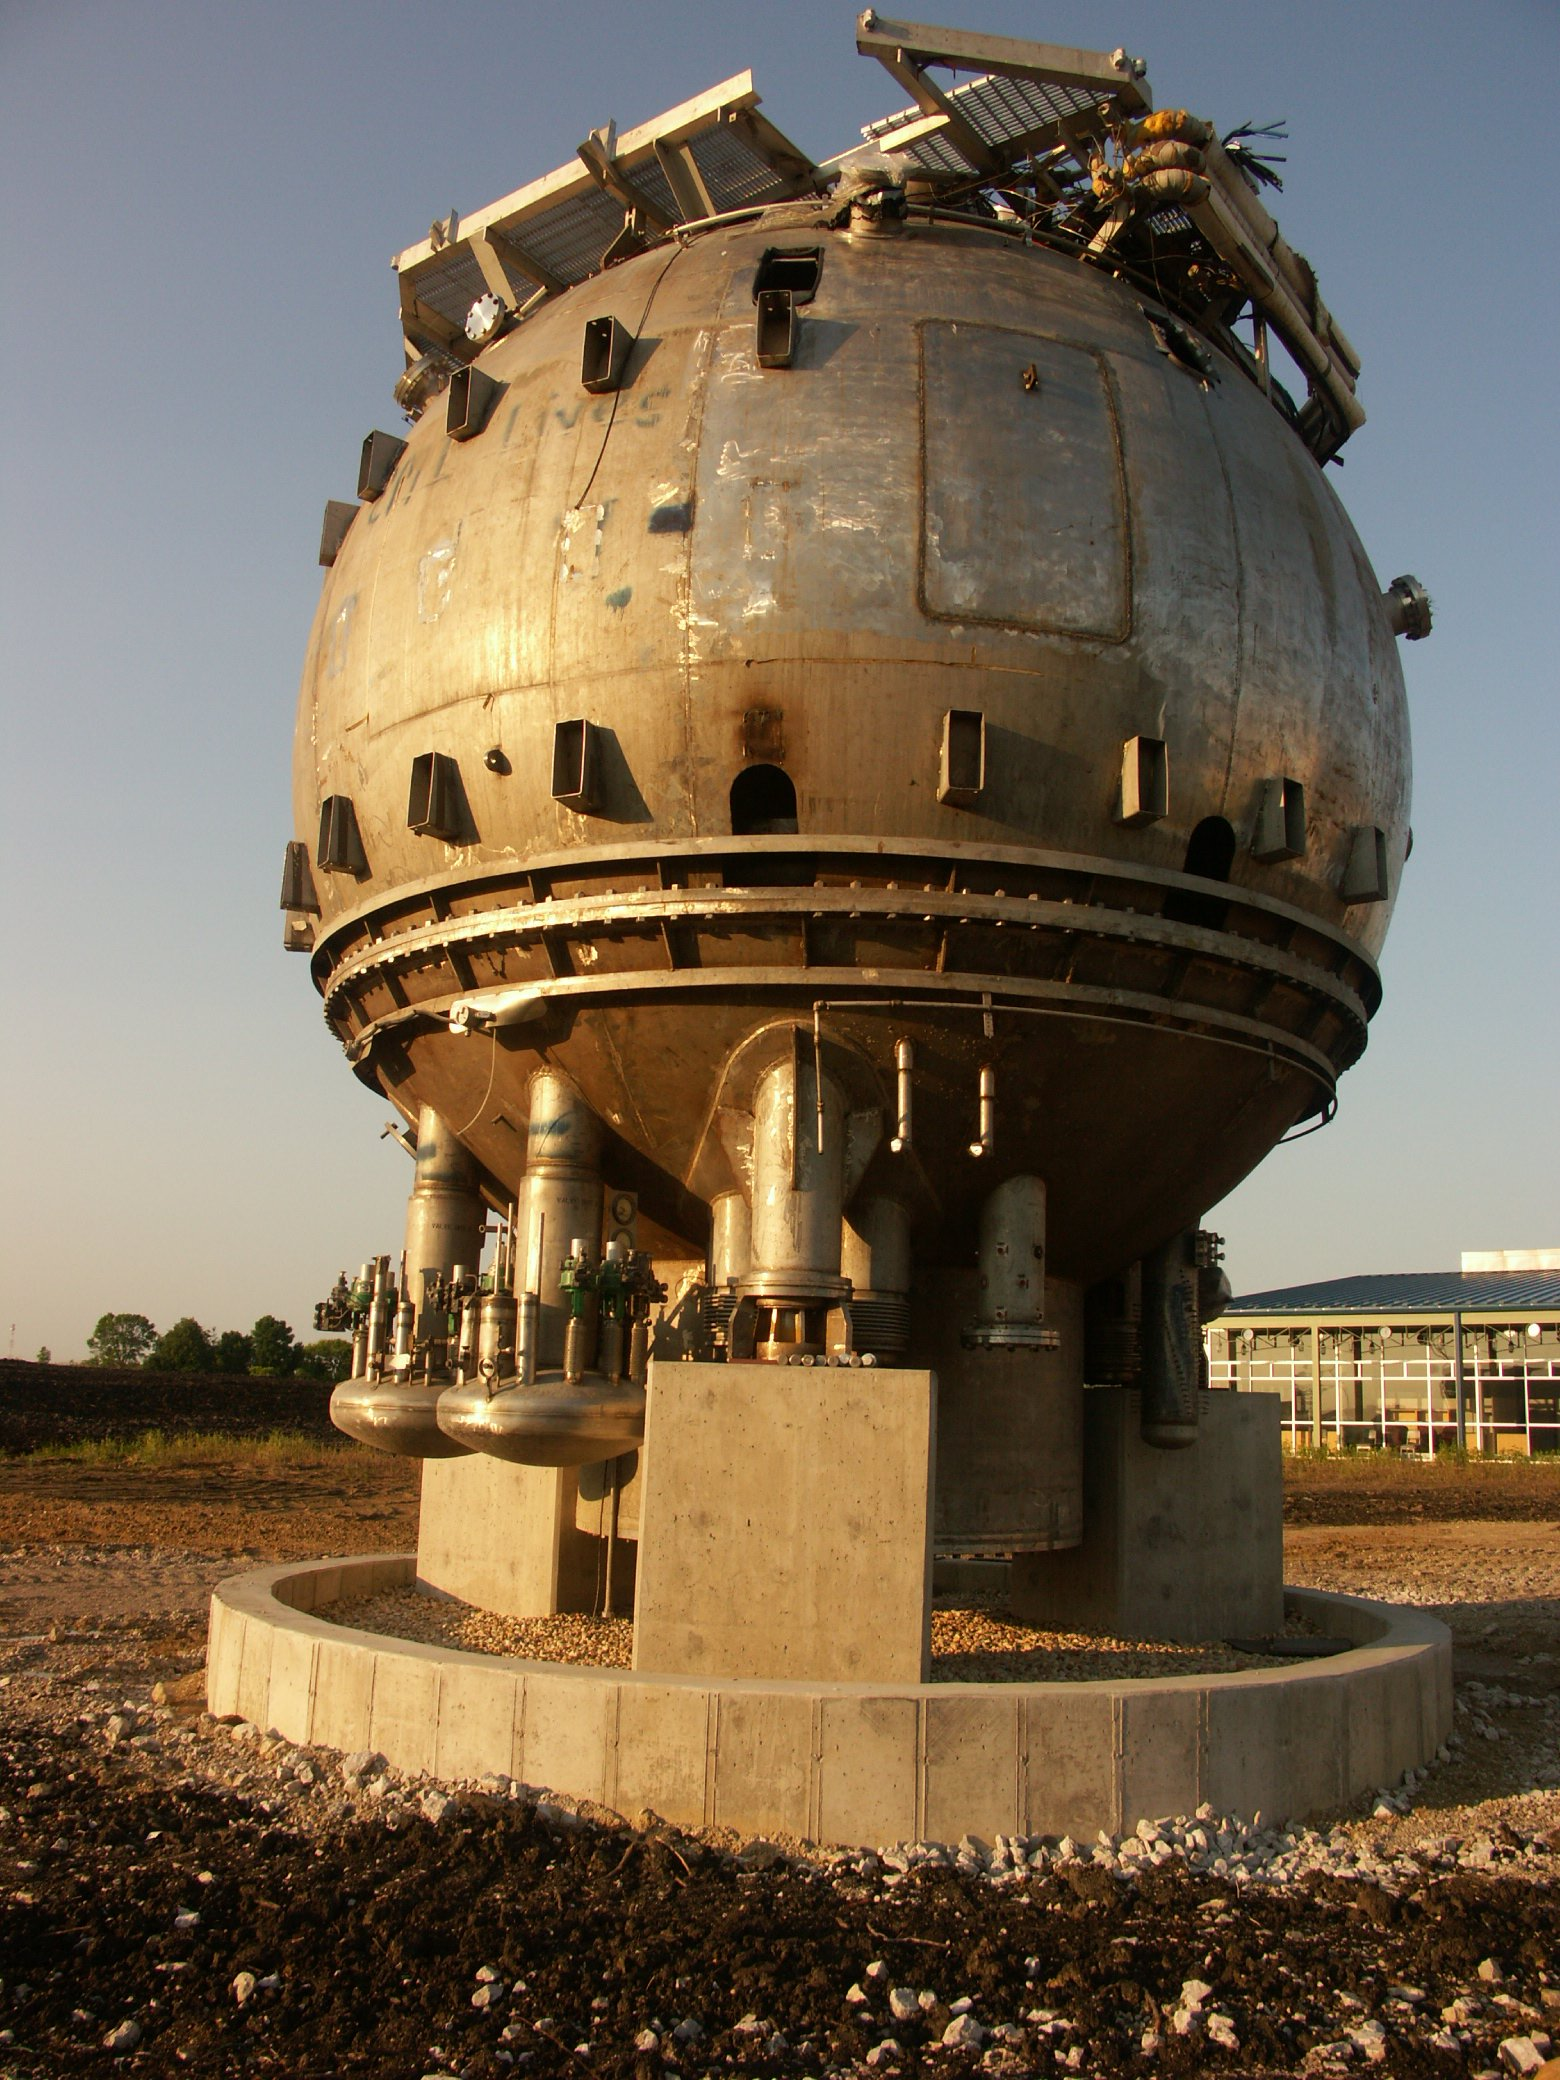
\includegraphics[width=0.5\linewidth]{./figures/bubblechamberfnal.jpg}
	\caption{An old bubble chamber, once used at Fermilab,
	 \cite{FNALBubbleChamber2005}}
	\label{fig:bubble_chamber}
\end{figure}

Invented by Donald Glaser in 1952, the bubble chamber was `perfected' by Luis
Alvarez when he helped to develop a version which could be used with liquid
hydrogen. Hydrogen was desirable as a target and medium due to its simple
structure. This led to cleaner results, unlike the original medium Ether.
Additionally, using hydrogen gave physicists a convenient way to directly probe
the sub-nuclear structure of the simplest form of matter.

\begin{figure}[ht]
	\centering
	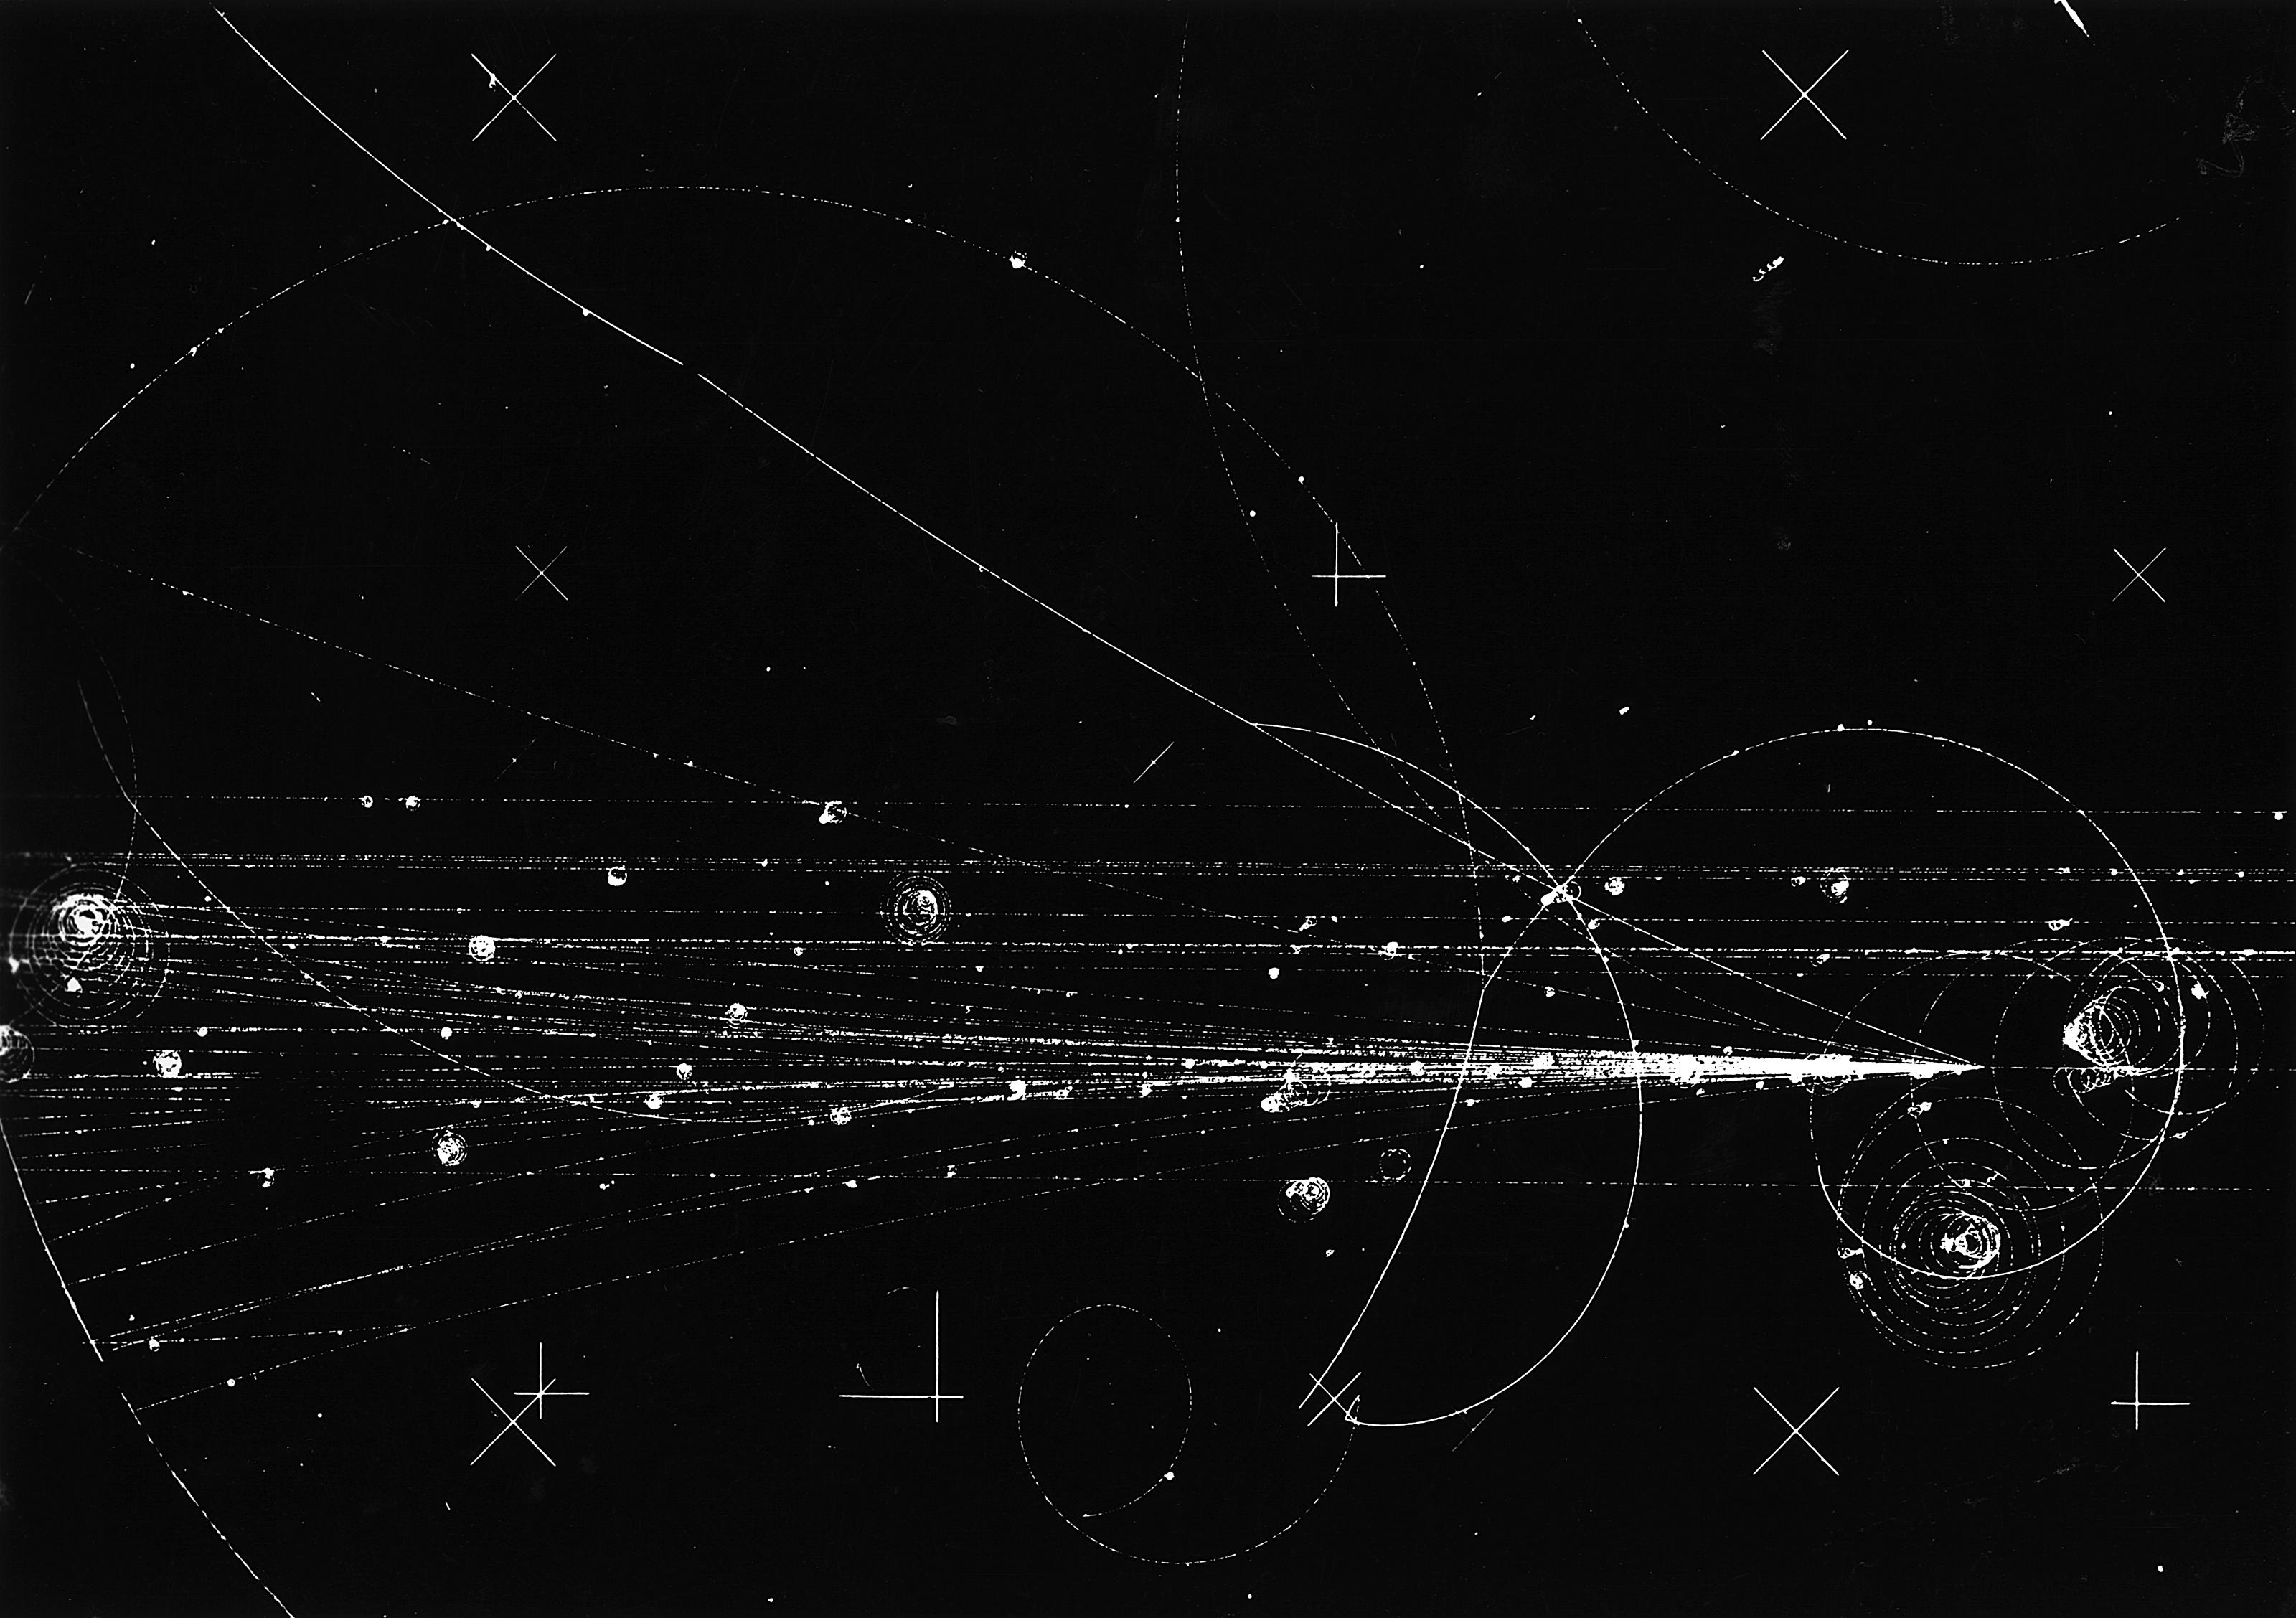
\includegraphics[width=0.5\linewidth]{./figures/bubble_chamber_tracks.jpg}
	\caption{
		An example of the photographs taken with a Bubble Chamber, in 1973.
		In this picture, we see a 300 $GeV$ proton producing particles as it travels
		through a hydrogen-filled bubble chamber at Fermilab  \cite{HD6B235}.
	}
	\label{fig:bubble_tracks}
\end{figure}

Soon after the advent of bubble chambers, physicists were able to
macroscopically image these new, exotic particles interacting with normal matter
and decaying. Novel computer techniques were developed to analyze and catalog
the massive influx of data.

A break-through came in 1961, when Gell-Mann and Nishijima recognized the
underlying symmetry of the interactions taking place and created what would be
known as `the eightfold way'. This theory created a scheme for organizing the
observed baryons and mesons according to their properties in groupings called
``octets''. These octets were in fact representations of the elements of members
of the $SU(3)$ group. Gell-Mann had discovered the underlying structure of
flavor-symmetry between the three lightest quarks--$u$, $d$, and $s$. 

Gell-Mann's quark model soon made important predictions which were later
verified, notably the existence of the $\Omega^{-}$ mesons, the ground-state
particle of the spin-$3/2$ decuplet, discovered at Brookhaven National
Laboratory. Gell-Mann formalized his quark theory of matter in 1964, however,
due to the unforeseen phenomena of color confinement, it would be several years
before evidence of quarks composing baryons and mesons was directly obtained
from deep inelastic scattering experiments.

This work directly led to the development of the quark model of matter and the
foundation of what would become the foundation of the standard model of
particles. To date, the standard model is the most successful theory describing
particles and their interactions.


\clearpage
\section{Deep Inelastic Scattering, Quantum Chromodynamics and The Parton Model}

Deep inelastic scattering experiments (Figure~\ref{fig:disschematic}) were a
natural outgrowth of Rutherford's experiment from the late 19th century.
Rutherford's scattering experiments can be modeled classically, by using a
classical potential as a scattering source. One solves as usual using an
impact parameter and potential as in central force problems.  Rutherford's
experiments were considered generally `elastic' because the target absorbed very
little kinetic energy from the projectile, and no new particles were created
from the kinetic energy of the projectile-target system.

By the late 20th century, scattering experiments became highly inelastic.
Targets would absorb a lot of kinetic energy, sometimes so much that targets
would break apart and the kinetic energy of the system would create particles.

Deep Inelastic scattering describes the process in which a high energy
interaction occurs between a projectile (often a beam) and a target (a gas, or
another beam). The process is akin to smashing to swiss-watches together to
understand how the gears fit together in synchrony to tell time. 

The interaction occurring between the target and the projectile can change the
state of the projectile and generate matter due to the high energies involved.
One can observe the state of the projectile and account for the matter which is
created.  If there are laws which govern how the state of the projectile changes
or the kinds of matter that can be created, then we can run the clock backwards
and reconstruct the initial state from the final state of the interaction.
Alternatively, the goal of deep inelastic scattering may also be to simply
measure and characterize the final state of an interaction, based on a known
initial state. This process teaches us something about nuclear structure (or
even partonic structure). In this way, one can also identify conserved
quantities, which in turn suggest physical symmetries and help to build models.

One can think of an interaction of a beam and target in terms of a probability
of interaction. One can mathematically `separate' part of this interaction
probability into a quantity called a 'cross-section', often denoted as $\sigma$
for a total cross section, or $d\sigma$ for a differential cross section, or
even ${d\sigma}\over{d\Omega}$ to refer to a differential cross section
scattered into a solid angle. Understanding the cross-section of a process
requires knowledge of the luminosity (interactions per second, per unit area) of
beam with respect to the target. Understanding Luminosity is of fundamental
importance, and is discussed in Chapter~\ref{ch:vernier_analysis}.

A subcategory of deep inelastic scattering is 'Semi-Inclusive Deep-Inelastic
Scattering'. This refers to a case where a beam (say a lepton, such as an
electron) interacts inelastically with a point-like internal structure of a
target particle, and a hadron is produced (such as a $\pi^+$), which is then
detected. Semi-Inclusive Deep-Inelastic scattering is then the process by which
the scattered lepton and a specific hadron are measured in the final state of
the interaction (but other particles that might be produced are neglected or
ignored).

Nuclei are not elementary particles. They are built up from what we assume are
fundamental particles. Deep inelastic scattering experiments slowly revealed
that individual protons and neutrons are not elementary particles, but instead,
composite particles.  It is natural to assume that the properties of protons and
neutrons are not `fundamental' either, in that these properties must be emergent
from the partonic substructure. In fact, the vast zoo of particles that were
discovered in early inelastic scattering experiments, such as $\pi$ or $K$, or
any meson or baryon are not fundamental, but bound states of quarks and gluons.

\begin{figure}[ht]
	\centering
	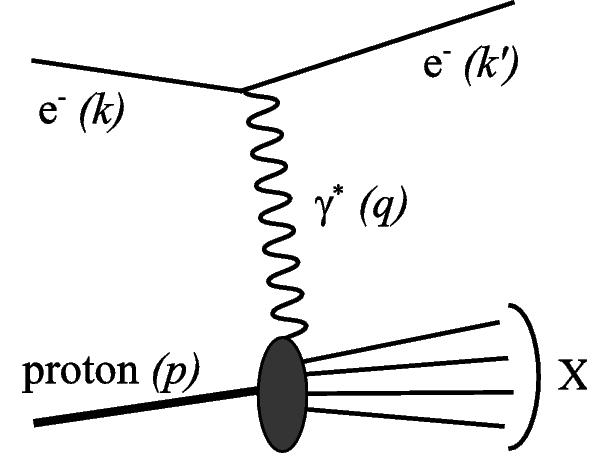
\includegraphics[width=0.6\linewidth]{./figures/deep_inelastic_basic.png}
	\caption{
    A schematic~\cite{Ddn2_2008} of deep inelastic scattering, where the
    incoming electron inelastically scatters off the proton, producing results
    $X$, via virtual photon exchange, $\gamma^*$. The diagram is split into a
    perturbative portion (the electron) and a non-perturbative portion.
    Mathematically, we describe the interaction with kinematic variables
    summarized in Equations~\ref{eq:P}-\ref{eq:x}
  }
	\label{fig:disschematic}
\end{figure}

By the 1970s, collaborations between Bjorken, Feynman, and others had produced
a coherent partonic model which contained quarks and force-mediating gluons.
The concept of Structure functions had been developed. Modified from
Rutherford's original scattering formula, a new formalism to describe the cross
section of deep inelastic scattering incorporated structure functions. Structure
Functions provide a means to separated out the momentum exchange between target
and projectile (via a virtual photon), and isolated this known process from the
total interaction. The $W_1$ and $W_2$, structure functions were defined to be
experimentally measured quantities representing the electron-proton
interaction~\cite{Riordan1992}.

This period of time, from 1970--1990 was truly the golden age of Deep Inelastic
Scattering Experiments. The biggest laboratories responsible for data from this
period were The European Organization for Nuclear Research (CERN), The Stanford
Linear Accelerator Center (SLAC), and The German Electron Synchrotron (DESY).
Thousands of ground-breaking papers were published, such as the CERN's European
Muon Collaboration experiment which showed a measurement of the spin asymmetry
and determination of the proton structure function $g_1$ in muon-proton deep
inelastic scattering \cite{Ashman1988}. 

The formalism of scattering theory continued to evolve during this booming
period.  Though the process of scattering itself has not changed since its
inception in Rutherford's lab, vast improvements in technology have allowed
unprecedented scattering energies with high luminosity accelerators. We now can
take measurements of particles and their properties with exquisite precision.
The level of precision now possible is exemplified in Brookhaven National
Laboratory's E821 Muon ($g$-$2$) experiment--which measured the anomalous
magnetic moment, $g$-$2$, of the muon to a precision of 7 parts in ten
million~\cite{Bennett}.

\clearpage

With the advent of the structure function model, we began an era where matter
ceased to be modeled as a simplistic bound-state of quarks, such as the valence
quark model for the proton, and instead, complex clouds of quark and gluon
interactions. The mathematics of scattering formalism had to change to
accommodate the underlying physical distribution of partonic matter in baryons.
Deep Inelastic Scattering continued to probe various portions of these structure
functions, and the structure of the standard model began to come into focus,
distilled into the relatively simple mathematical structure of group theory. The
standard model is a gauge theory, which contains the internal symmetries of
$SU_{c}(3) \times SU_{L}(2) \times U_{Y}(1)$ (Figure~\ref{fig:standardmodel}).
The Standard Model is said by some to be ``complete'' with the discovery of the
Higgs Boson, yet for emergent phenomena such as proton spin, it does not provide
a straightforward prediction. 

\begin{figure}[ht]
	\centering
	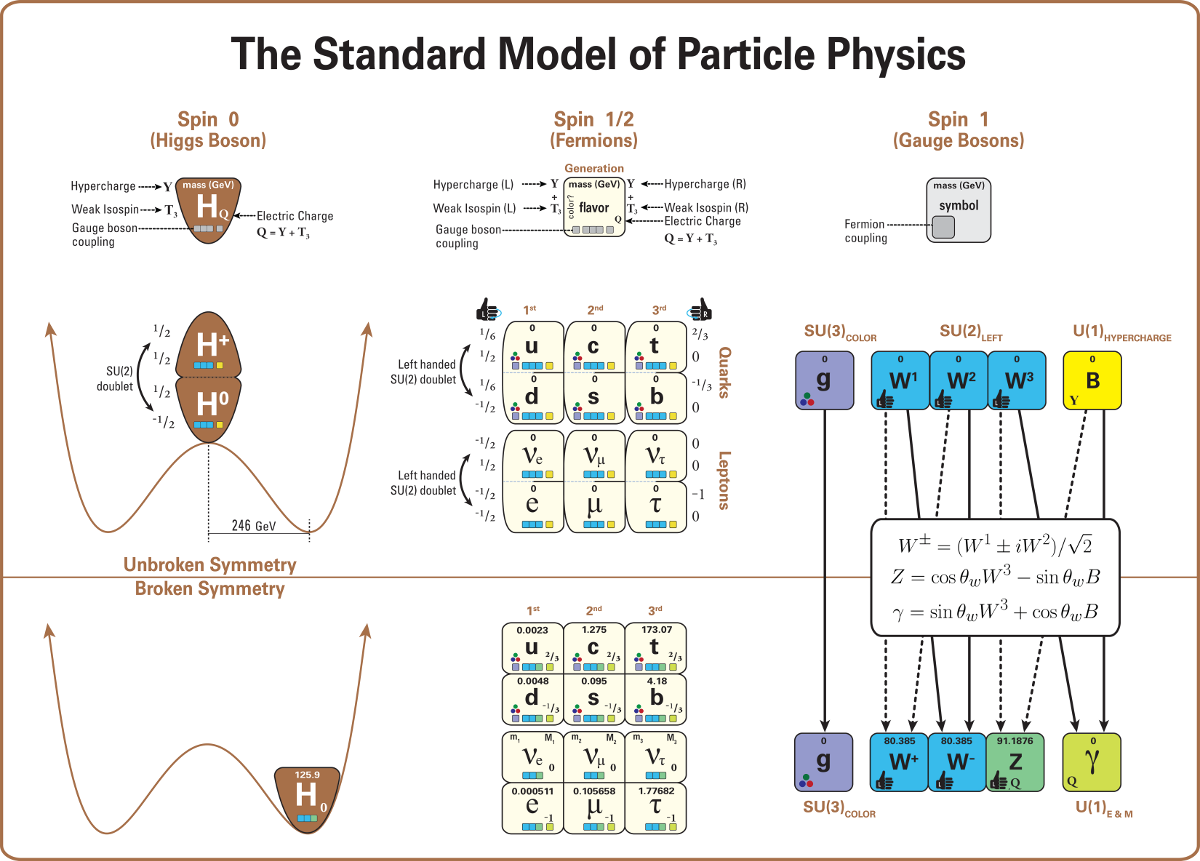
\includegraphics[width=\linewidth]{./figures/standard_model_complete_lowres.png}
	\caption{
		``This diagram displays the structure of the standard model (in a way that
		displays the key relationships and patterns more completely, and less
		misleadingly, than in the more familiar image based on a 4x4 square of
		particles). In particular, this diagram depicts all of the particles in the
		standard model (including their letter names, masses, spins, handedness,
		charges, and interactions with the gauge bosons -- i.e. with the strong and
		electroweak forces). It also depicts the role of the Higgs boson, and the
		structure of electroweak symmetry breaking, indicating how the Higgs vacuum
		expectation value breaks electroweak symmetry, and how the properties of the
		remaining particles change as a consequence.''\cite{Boyle2014}.
	}
	\label{fig:standardmodel}
\end{figure}


\clearpage
\section{Modern Deep Inelastic Scattering Experiments}

Here, I hope to highlight the last 40 years or so of physics produced by deep
inelastic scattering experiments. The boundaries of science are pushed by huge
collaborations of men and women working together, starkly contrasting the lonely
pursuits of a handful of scientists in 19th century laboratories.

This era of deep inelastic scattering has unearthed some of the most surprising
and monumental discoveries in physics, from the recent discovery of the
Higgs-particle, to the discovery that protons and neutrons are not fundamental
particles at all, but are instead, highly relativistic balls of gluons.

SLAC Experiments (E80-E155) were some of the first experiments to probe the
proton spin structure, operating from 1978-1999. SLAC pioneered the usage of
spin asymmetries as a means of ruling out models for various parameterizations
of quark structure functions, as well as provided important data constraining
nuclear structure functions. SLAC's experiments focused on understanding the
spin structure of the quarks (but not gluons) within protons.

The European Muon Collaboration at CERN was one of the first major international
efforts to study the underlying structure of protons and neutrons with deep
inelastic scattering. The collaboration produced scientific results from 1979 to
1997. The EMC's major contribution to our understanding of nuclear structure was
to amass evidence which supported the parton model of protons and neutrons, as
well as discovering the self-named `EMC effect', which showed that the volume
`occupied' by quarks scales with heavier nuclei~\cite{Aubert1983}. EMC also
elucidated the effects of quark fragmentation and hadron production, DIS in the
nuclear medium, and produced some of the first measurements of the spin
structure of the proton. Most famously, the EMC originally published the `proton
spin crisis' in its first measurement of the proton spin structure function,
$g1$ where it found the spin carried by the proton's 'valence quarks' is
significantly less than $1/2$~\cite{Ashman1988}. 

CERN produced another collaboration which contributed to our understanding of
nuclear structure, the Spin Muon Collaboration. SMC was active from 1993 to 1998
and used polarized beams of muons to interact with a spin polarized target
(ammonia and later p-butanol). SMC measured virtual photon production
asymmetries, $A_1$, in order to measure information about the proton spin
structure function, $g_1$ (discussed in detail in the following chapter). $g_1$
gives access to the quark polarization of protons. Spin structure physics has
been explored at the COMPASS experiment since 2005. CERN's work to understand
the spin structure of the proton probed the contributions of both the quark, and
gluons. 

The German Electron Synchrotron (DESY) is Germany's the premier accelerator
science laboratory, and has been operating continuously since 1964. DESY's
primary experiments in deep inelastic scattering to understand nuclear structure
have been underway since 1992. DESY operates several deep inelastic scattering
experiments including ZEUS, HERA (H1 and H2) and HERMES.  The scientific goals
of the DESY institute as a whole are broad, since it represents Germany's
premier accelerator physics scientific effort. DESY hosts experiments in
condensed matter physics and astrophysics, addition to its efforts in DIS.
However, the portion of DESY's research program devoted to spin structure seeks
to understand both the quark and gluon contributions to proton spin.

Jefferson Laboratory (JLab) is an electron accelerator complex in Virginia
specializing in the cutting edge of fixed target electron deep inelastic
scattering experiments. Experiments in Hall A, B and C are all involved with
studying both quark and gluon contributions to proton spin.

Finally, there is the Relativistic Heavy Ion Collider, and the experiment
PHENIX. RHIC and PHENIX are discussed in detail in
Chapter~\ref{ch:experimental_apparatus}. This thesis presents an analysis of the
data set recorded in 2013 by the PHENIX detector.
